Since our harvesting control is proportional to our population, given a finite time horizon $T$, the amount of fishes we have extracted from our pool is given by,
\begin{align}
	J(x;p,T)&=\int_{0}^{T} p x \diff{t} \nonumber \\
			&=\int_{0}^{T} \frac{M p\left(r-p\right)x_0}{rx_0+\left(M\left(r-p\right)-rx_0\right)\euler^{-(r-p) t}} \diff{t} \nonumber
\end{align}
The equation \ref{eq: Proportional Population} determines the population of fishes at time $t$. Consider the transformations $y=x/M$, $\tau=rt$, $\bar{p}=rp$. Therefore the equation \ref{eq: PropHarvest}, is transformed into:
\begin{equation}
\dev{y}{\tau}=(1-\bar{p})y\left(1-\frac{y}{1-\bar{p}}\right)
\end{equation}
with initial condition $y(0)=y_0=x_0/M$. And solution,

\begin{equation}
	y(\tau)=\frac{(1-\overline p)y_0}{y_0+\left(1-\overline p-y_0\right)\euler^{(\overline p-1)\tau}}
\end{equation}
Then our function in the time horizon $\bar{T}=rT$
\begin{align}
J\left(y;\bar{p},\bar{T}\right)&=\frac{1}{rM}\int_0^{\bar{T}}\bar{p}y(\tau)\diff{\tau}	\\
&=\frac{\bar{p}}{rM}\left(\ln\left(1-\bar{p}+y_0\left(\euler^{(1-\bar{p})\bar{T}}-1\right)\right)-\ln\left(1-\bar{p}\right)\right)
\end{align}

We would like to know the constant $\bar{p}^*$ that for a given time horizon $\bar{T}$ maximizes $J$. Therefore $\bar{p}$ should satisfy the necessary condition,
\begin{equation}
\left.\pdev{J\left(y;\bar{p},\bar{T}\right)}{p}\right|_{\bar{p}=\bar{p}^*}=0
\end{equation}

Therefore, for given $y_0$ we need to solve for $\bar{p}^*$ the following equation,
\begin{equation}
\bar{p}^* \left(\frac{1+Ty_0\euler^{\left(1-\bar{p}^*\right)\bar{T}}}{\bar{p}^*+y_0-1 -y_0\euler^{(1-\bar{p}^*)\bar{T}}}+\frac{1}{1-\bar{p}^*}\right)+\ln
\left(1-\bar{p}^*-y_0 +y_0\euler^{(1-\bar{p}^*)\bar{T}}\right)-\ln\left(1-\bar{p}^*\right)=0 \label{eq: Nonlinear equation}
\end{equation}

This expression has no closed form solution, but we can estimate it numerically, if we know $y_0$ and $T$. For example for $y_0=0.75$ and $\bar{T}=20$, we have
$\bar{p}^* \approx 0.541881$.


Given a time horizon $\bar{T}=24$ time units (usually given in months), above with parameters $M=780500$ fishes, $r=0.8$ inverse time units and initial population $x_0=390250$. The following numerical results are done with $\bar{p}^*\approx 0.531176$ given by the equation \ref{eq: Nonlinear equation}. 

\begin{figure}[H]
	\centering
	\begin{subfigure}[b]{0.45\textwidth}
		\centering
		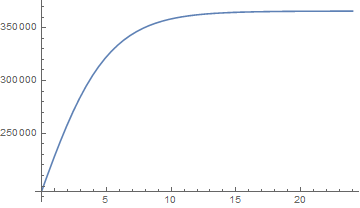
\includegraphics[width=0.9\textwidth]{optpop.png}
		\caption{Population with optimal $p^*$. }		
	\end{subfigure}
	\begin{subfigure}[b]{0.45\textwidth}
		\centering
		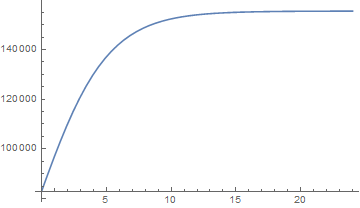
\includegraphics[width=0.9\textwidth]{optpro.png}
		\caption{Harvest Fishes taken with optimal $p^*$.}
	\end{subfigure}
\end{figure}

The first graph show the total population of fishes during the time, and the second one represent the amount of fishes that are harvest from the model. As we can see the population goes to an stability point that is equal to $\left(1-\frac{p}{r}\right)M$ and in the same way the amount of fishes that we harvest goes to $\bar{p}^*\left(1-\bar{p}\right)M$. The following graphs shows the variation $\bar{p}^*\pm0.1$  an the effect in the amount of harvested fish, please note how the stable fixed points lie below $M/2$:
\begin{figure}[H]
	\centering 
	\begin{subfigure}[b]{0.45\textwidth}
		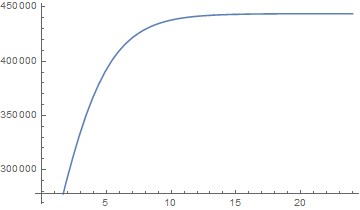
\includegraphics[width=0.9\linewidth]{lshpop.png}
		\caption{Population with $\bar{p}^*-0.1$}		
	\end{subfigure}
	\begin{subfigure}[b]{0.45\textwidth}
		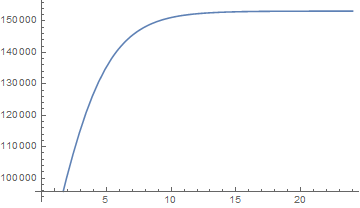
\includegraphics[width=0.9\linewidth]{lshpro.png}
		\caption{Harvest fish rate with $\bar{p}^*-0.1$}			
	\end{subfigure}
	\begin{subfigure}[b]{0.45\textwidth}
		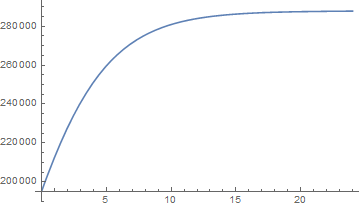
\includegraphics[width=0.9\linewidth]{mrhpop.png}
		\caption{Population with $\bar{p}^*+0.1$}			
	\end{subfigure}
	\begin{subfigure}[b]{0.45\textwidth}
		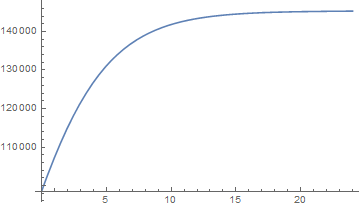
\includegraphics[width=0.9\linewidth]{mrhpro.png}
		\caption{Harvest fish rate with $\bar{p}^*+0.1$}			
	\end{subfigure}
\end{figure} 

In the first two there is less harvesting, then the population is bigger, but since the harvesting coefficient is smaller the amount of fishes is smaller. In the other hand, when the harvesting coefficient is bigger the population is smaller, since the harvested fish is proportional to the population, then we harvest less fish. We see the above explained behavior in table \ref{tab: OptimumHarvestFish} in contrast with the optimum, corresponding to some specific parameters. 
\begin{table}[H]
	\begin{center}
	\begin{tabular}{@{}l|r@{}}
		\rowcolor[HTML]{E5FDCB} 
		\textbf{$\bar{p}$}            & \textbf{\begin{tabular}[c]{@{}r@{}}$J(x;T,p,r,M,x0)$\\ (in Millions of fishes harvested)\end{tabular}} \\
		\toprule
		\rowcolor[HTML]{CEFB9C} 
		$ \bar{p}^*$& 4.698153484016761                                                                                    \\
		\rowcolor[HTML]{E2F7E2} 
		$\bar{p}^*-0.001$             & 4.698138002580389                                                                                    \\
		\rowcolor[HTML]{E2F7E2} 
		$\bar{p}^*+0.001$             & 4.698138014054768                                                                                    \\
		\rowcolor[HTML]{E2F7E2} 
		$\bar{p}^*-0.01$              & 4.696602091505628                                                                                    \\
		\rowcolor[HTML]{E2F7E2} 
		$\bar{p}^*+0.01$              & 4.696609852932111                                                                                    \\
		\rowcolor[HTML]{E2F7E2} 
		$\bar{p}^*-0.1$               & 4.540022027777682                                                                                    \\
		\rowcolor[HTML]{E2F7E2} 
		$\bar{p}^*+0.1$               & 4.547918150118066                                                                                    \\ \bottomrule
	\end{tabular}
	\caption{Harvested fish $J(x; \bar{p}, T, M, r, x_0)$ in units of million of fishes  with different $\bar{p}$, for $T=24$, $r=0.8$, $M=780500$, $x_0=390250$}
	\label{tab: OptimumHarvestFish}
\end{center}
\end{table}

We can know estimate the value of $\bar{p}^*$, for long time horizons. Consider,  
\begin{equation}	
\lim\limits_{T\rightarrow \infty} \ln(a+b\euler^{cT})\approxeq cT
\end{equation}

For any $a,b \in \mathbb{R}$. And
\begin{equation}
	\lim\limits_{T-\infty}\frac{a+bT\euler^{cT}}{r+d\euler^{cT}} \approxeq \frac{b}{d}T
\end{equation}
For any constants $a,b,c,d,r \in \mathbb{R}$. 

Therefore, for big enough $T$, the contribution for fixed $\bar{p}^*$, we can write equation \ref{eq: Nonlinear equation} in small-$o$ notation as follows,
\begin{equation}
\lim\limits_{T\rightarrow \infty}\left.\pdev{J}{p}\right|_{p=\bar{p}^*} =(1-\bar{p}^*)\bar{T}-\bar{p}^*\bar{T}+o(T)+o(T^2)+\dots=0 
\end{equation}

Hence, when $T\rightarrow \infty$
\begin{equation}
	(1-2\bar{p}^*)\bar{T}=0\implies \bar{p}^*=\frac{1}{2}
\end{equation}

This result was expected, since 
$\lim\limits_{T\rightarrow\infty} x(t) = r\bar{p}(1-\bar{p})M$, for any initial condition $x_0$. Therefore, for long time horizons $T\rightarrow \infty$, the functional $J(x; T,\bar{p},r,M)\rightarrow r\bar{p}(1-\bar{p})MT$, becomes a concave function of $\bar{p}^*$, whose maximum is reached at the point $\bar{p}^*=\frac{1}{2}$.